\documentclass[12pt]{article}
\usepackage[T1, T2A]{fontenc}
\usepackage[utf8]{inputenc}
\usepackage[russian]{babel}
\usepackage{hyperref}
\usepackage{graphicx}
\graphicspath{ {../Images/} }

\author{Григорий Матюхин}
\date{\today}
\title{Лабораторная работа \textnumero13.\\Фильтр пакетов}

\begin{document}
\maketitle
\newpage
\tableofcontents
\newpage
\section{Цель работы}
Получить навыки настройки пакетного фильтра в Linux.

\section{Последовательность выполнения работы}
\subsection{Управление брандмауэром с помощью \texttt{firewall-cmd}}
\begin{enumerate}
	\item Получите полномочия администратора:
	\item Определите текущую зону по умолчанию:
	\item Определите доступные зоны:
	      \\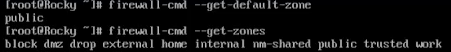
\includegraphics{1.png}
	\item Посмотрите службы, доступные на вашем компьютере:
	      \\
\includegraphics{2.png}
	\item Определите доступные службы в текущей зоне:
	      \\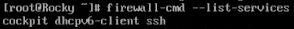
\includegraphics{3.png}
	\item Сравните результаты вывода информации при использовании команды
	      \texttt{firewall-cmd --list-all}
	      и команды
	      \texttt{firewall-cmd --list-all --zone=public}:
	      \\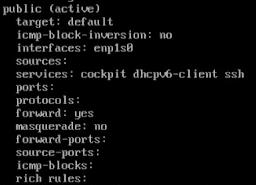
\includegraphics{4.png}
	\item Добавьте сервер VNC в конфигурацию брандмауэра:
	      \\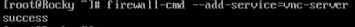
\includegraphics{5.png}
	\item Проверьте, добавился ли vnc-server в конфигурацию:
	      \\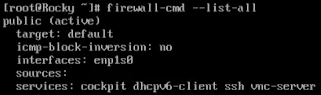
\includegraphics{6.png}
	\item Перезапустите службу firewalld:
	\item Проверьте, есть ли vnc-server в конфигурации:
	      \\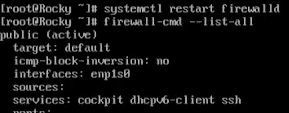
\includegraphics{7.png}
	\item Добавьте службу vnc-server ещё раз, но на этот раз сделайте её постоянной
	\item Поверьте наличие \texttt{vnc-server} в конфигурации:
	      \\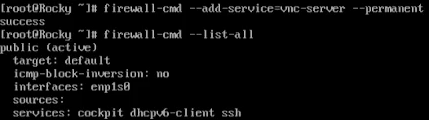
\includegraphics{8.png}
	\item Перезагрузите конфигурацию \texttt{firewalld} и просмотрите конфигурацию времени выполнения:
	      \\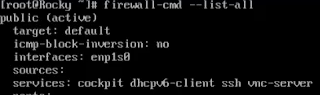
\includegraphics{9.png}
	\item Добавьте в конфигурацию межсетевого экрана порт 2022 протокола TCP:
	      \\
\includegraphics{10.png}
	\item Проверьте, что порт добавлен в конфигурацию:
	      \\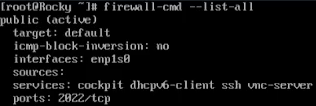
\includegraphics{11.png}
\end{enumerate}

\subsection{Управление брандмауэром с помощью \texttt{firewall-config}}
\begin{enumerate}
	\item Откройте терминал и под учётной записью своего пользователя запустите интерфейс GUI \texttt{firewall-config}:
	\item Нажмите выпадающее меню рядом с параметром Configuration. Откройте раскрывающийся список и выберите Permanent. Это позволит сделать постоянными все изменения, которые вы вносите при конфигурировании.
	\item Выберите зону \texttt{public} и отметьте службы \texttt{http}, \texttt{https} и \texttt{ftp}, чтобы включить их.
	      \\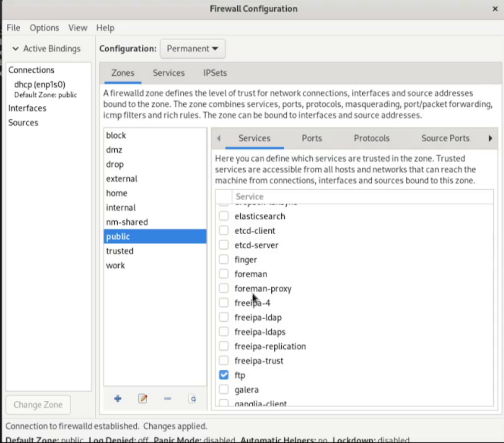
\includegraphics{12.png}
	\item Выберите вкладку Ports и на этой вкладке нажмите Add. Введите порт 2022 и протокол \texttt{udp}, нажмите ОК, чтобы добавить их в список.
	      \\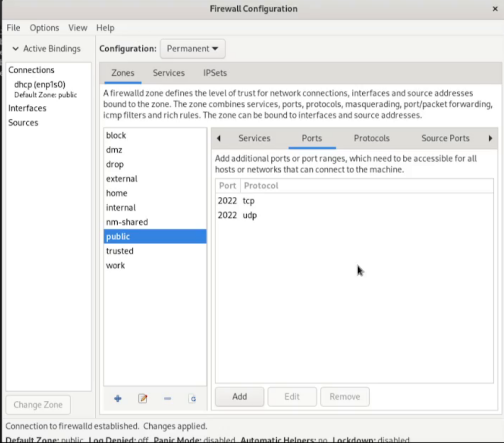
\includegraphics{13.png}
	\item Закройте утилиту \texttt{firewall-config}.
	\item Просмотрите конфигурацию времени выполнения:
	\item Перегрузите конфигурацию \texttt{firewall-cmd} и посмотрите еще раз:
	      \\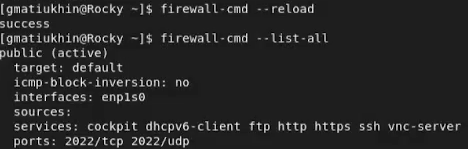
\includegraphics{14.png}
\end{enumerate}

\subsection{Самостоятельная работа}
\begin{enumerate}
	\item Создайте конфигурацию межсетевого экрана, которая позволяет получить доступ
	      к следующим службам:
	      \begin{itemize}
		      \item telnet;
		      \item imap;
		      \item pop3;
		      \item smtp.
	      \end{itemize}
	      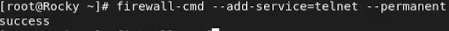
\includegraphics{15.png}
	\item Сделайте это как в командной строке (для службы \texttt{telnet}), так и в графическом
	      интерфейсе (для служб \texttt{imap}, \texttt{pop3}, \texttt{smtp}).
	      \\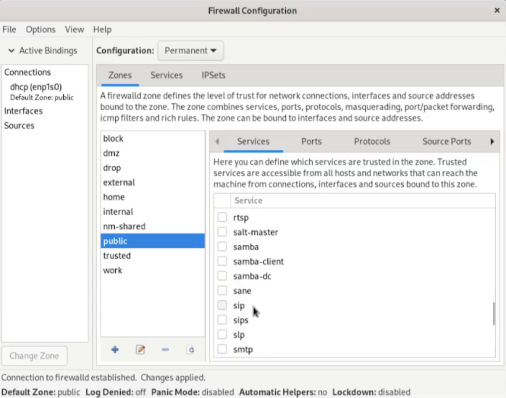
\includegraphics{16.png}
	\item Убедитесь, что конфигурация является постоянной и будет активирована после перезагрузки компьютера.
	      \\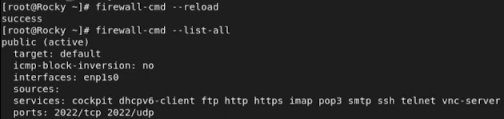
\includegraphics{17.png}
\end{enumerate}

\section{Контрольные вопросы}
\begin{enumerate}
	\item Какая служба должна быть запущена перед началом работы с менеджером конфигурации брандмауэра \texttt{firewall-config}? \\
	      \texttt{firewalld}
	\item Какая команда позволяет добавить UDP-порт 2355 в конфигурацию брандмауэра в зоне по умолчанию? \\
	      \texttt{firewall-cmd --add-port=2355/udp}
	\item Какая команда позволяет показать всю конфигурацию брандмауэра во всех зонах? \\
	      \texttt{firewall-cmd --list-all}
	\item Какая команда позволяет удалить службу \texttt{vnc-server} из текущей конфигурации брандмауэра? \\
	      \texttt{firewall-cmd --remove-service=vnc-server}
	\item Какая команда \texttt{firewall-cmd} позволяет активировать новую конфигурацию, добавленную опцией --permanent? \\
	      \texttt{firewall-cmd --reload}
	\item Какой параметр \texttt{firewall-cmd} позволяет проверить, что новая конфигурация была добавлена в текущую зону и теперь активна? \\
	      \texttt{--list-all}
	\item Какая команда позволяет добавить интерфейс \texttt{eno1} в зону \texttt{public}? \\
	      \texttt{firewall-cmd --add-service=eno1 --zone=public}
	\item Если добавить новый интерфейс в конфигурацию брандмауэра, пока не указана зона, в какую зону он будет добавлен? \\
	      В зону по умолчанию. Узнать текущую зону по умолчанию можно с помощю команды \texttt{firewall-cmd --get-default-zone}, а поменять с помищью \texttt{firewall-cmd --set-default-zone=<new-default-zone>}
\end{enumerate}

\section{Вывод}
В ходе выполнения данной работы я получил навыки настройки пакетного фильтра в Linux.

\end{document}
